\documentclass[11pt]{article}
\usepackage[letterpaper,centering,top=1in,total={6.5in,9in}]{geometry}
\usepackage{color}
\usepackage{graphicx}
\usepackage{listings}
\usepackage{hyperref}
%\usepackage{draftwatermark}
%\SetWatermarkScale{4.0}

% setups and definitions of commands (fold)
\definecolor{linkblue}{rgb}{0.3,0.5,0.75}
\definecolor{lightblue}{rgb}{0.4,0.6,0.75}

\hypersetup{colorlinks=true, linkcolor=linkblue, urlcolor=linkblue }

\lstset{ %
	language=XML,                % choose the language of the code
	basicstyle=\small,       % the size of the fonts that are used for the code
	numbers=none,
	tabsize=2,
	breaklines=true,
	morekeywords={sbml, model, math, listOfQualitativeSpecies, qualitativeSpecies, listOfSymbolicValues, symbolicValue, listOfTransitions, transition, listOfInputs, input, listOfOutputs, output, listOfFunctionTerms, functionTerm, defaultTerm, temporisationMath, listOfCompartments, compartments, apply, and, ci, cn, or, eq, neq, geq, leg, gt, lt}
}


\newcommand{\ALL}{\noindent\fbox{\footnotesize \textbf{All}}\ }
\newcommand{\LRG}{\noindent\fbox{\footnotesize \textbf{LRG}}\ }
\newcommand{\SYM}{\noindent\fbox{\footnotesize \textbf{SYM}}\ }
\newcommand{\PN}{\noindent\fbox{\footnotesize \textbf{PN}}\ }
\newcommand{\sbml}[1]{\textsf{\textbf{#1}}} %def of sbml class names
\newcommand{\mathml}[1]{\texttt{\textbf{#1}}} %def of sbml class names
\newcommand{\attr}[1]{\textsf{#1}} %def of xml attributes
\newcommand{\const}[1]{\texttt{#1}} %def of xml constants
\newcommand{\type}[1]{\texttt{#1}} %def of xml/SBML types
\newcommand{\qualt}[1]{\textsf{\textbf{\hypertarget{#1}{#1}}}\textsf{\textbf{\hypertarget{#1s}{}}}} %def of sbml class names
\newcommand{\qual}[1]{\textsf{\textbf{\hyperlink{#1}{#1}}}} %call a L3F:qual class names
\newcommand{\listOf}[1]{\textsf{\textbf{\hyperlink{#1}{ListOf#1}}}} %call a L3F:qual class names

\newcommand{\Q}[1]{\indent\fbox{\textcolor{red}{Question: #1}} }
\newcommand{\A}[1]{\textcolor{lightblue}{Answer: #1} }
\newcommand{\TODO}[1]{\colorbox{lightblue}{\textcolor{white}{TODO: #1}}}

% setups and definitions of commands (end)

\begin{document}
% title and infos on versions (fold)
\fbox{	
\begin{minipage}[t]{0.9\columnwidth}

	\section*{Proposal title}
	Qualitative Models (qual)

	\section*{Proposal authors\footnote{Have also collaborated to this proposal: T. Helikar, A. von Kamp, S. Klamt, N. Le Nov\`ere}}
	Duncan Berenguier\\
	TAGC INSERM U928 and IML CNRS UMR 6206, \\
	Luminy, 163 av. de Luminy 13288 Marseille, France\\
	~\\
	Claudine Chaouiya\\
	IGC Rua da Quinta Grande, 6, P-2780-156 Oeiras, Portugal\\
	~\\
	Aurelien Naldi\\
	Center for Integrative Genomics , University of Lausanne\\
	Genopode Building, CH-1015 Lausanne, Switzerland\\
	~\\
	Denis Thieffry\\
	IBENS, 46 rue d'��ULM, 75005 Paris, France

	\section*{Proposal tracking number}
	\TODO{ask for a tracking number}
	

	\section*{Version information}
	\bigskip
\subsection*{Version number and date of public release}
	Version 2.1 released on May, 12, 2011%\today
	
	\bigskip
\subsection*{URL for this version of the proposal}
	\url{http://sbml.org/Community/Wiki/SBML_Level_3_Proposals/Qualitative_Models}

	\bigskip
\subsection*{URL for the previous versions of this proposal}
	\url{http://sbml.org/Events/Other_Events/Alternative_modelling_Frameworks_2008/L3F_Proposal}.
		\TODO{add previous proposal}

\end{minipage}
}
% title (end)
\section*{Introduction and motivation}
\bigskip
\subsection*{Motivation} % (fold)
Quantitative methods for modelling biological networks require an in-depth knowledge of the biochemical reactions and their stoichiometric and kinetic parameters. In many cases, this knowledge is missing. This has led to the development of several qualitative modelling methods using information such as gene expression data coming from functional genomic experiments. Qualitative models are typically based on the definition of \emph{regulatory} or \emph{influence graph}. The components of these models differ from species and reactions used in current SBML models. For example, qualitative models typically associate discrete levels of activities with entity pools; the processes involving them cannot be described as reactions per se but rather as transitions between states. Boolean networks, logical models and some Petri nets are the most used qualitative formalisms in biology. Despite differences from traditional SBML models, it is desirable to bring these classes of models under a common format scheme. The purpose of this Qualitative Models package for SBML Level 3 is to support qualitative models into SBML.

% motivation (end)
\bigskip
\subsection*{Past work on this problem or similar topics} % (fold)
After several attempts to use the existing SBML L2 format, a decision was made to develop an extension for SBML L3.
A first proposal written in August 2008 by Duncan Berenguier and Nicolas Le Nov\`ere was discussed during a meeting on the 12th and 13th of August 2008\footnote{Nicolas Le Nov\`ere (\href{http://www.sbml.org}{SBML}), Sarah Keating (SBML), Nicolas	Rodriguez (SBML), Denis Thieffry (\href{http://gin.univ-mrs.fr/}{GINsim}), Duncan Berenguier (GINsim), Aur\'elien Naldi (GINsim), Claudine Chaouiya (GINsim, Petri nets), Tomas Helikar (\href{http://www.bioinformatics.org/chemchains/wiki/}{Chemchains}), Ioannis Xenarios (\href{http://www.enfin.org/dokuwiki/doku.php?id=squad:start}{SQUAD}), Alessandro Di Cara (SQUAD), Mathias John (\href{http://piml.sourceforge.net/}{PiML}), Dagmar Koehn (PiML)}. 
%The previous proposal is available at \url{http://www.ebi.ac.uk/compneur/xwiki/bin/download/SBML/L3F/L3F_extension_draft_1.1.pdf}.
This meeting led to the release of a document (L3F\_extention\_draft\_1.2.pdf) which is a revision of a previous proposal for this package. A summary of the meeting is available at \url{http://www.ebi.ac.uk/compneur/xwiki/bin/view/SBML/L3F}, and a document 
\medskip
A second meeting was held at in November 2010 (see \url{http://compbio.igc.gulbenkian.pt/nmd/node/30}, for the program and participants). A revised version of the proposal was discussed during this meeting.
This document accounts for the outcomes of the meeting discussions and of following exchanges. 
% past work (end)

\bigskip
\subsection*{Graphical and typographical conventions} % (fold)

Throughout this document, the following typographical conventions are used :
\begin{itemize}
	\item \sbml{Classes} names begin with a capital letter a capital letter and are written in bold, sans-serif typeface. In addition, if a class describes elements introduced in this extension, these are written in light blue and are hyperlinked to the section where they are defined, \emph{e.g.} \qual{QualitativeSpecies}.
	\item \attr{attributes} are written in sans-serif typeface.
	\item \const{constants} and \type{types} are written in typewriter typeface.
\end{itemize}

As this proposal covers various formalisms, the examples are labeled with a token indicating the corresponding formalism : \ALL all formalisms, \PN Petri nets, \LRG logical regulatory networks or \SYM symbolic relationships.

% conventions (end)

\section*{XML Namespace} % (fold)

The XML-namespace used for elements defined by sbml-qual follows the convention of all SBML packages. This means that the namespace is "http://www.sbml.org/sbml/level3/version1/qual/version1" (in the case of SBML Level 3 version 1, SBML-qual version 1).

% XML namespace (end)

\section*{Proposed syntax and semantics} % (fold)

Like \sbml{Species} in SBML, the components of qualitative models refer to pools of entities that are considered indistinguishable and are each located in a specific \sbml{Compartment}. However, here components are characterised by their qualitative influences rather than by taking parts into reactions. Therefore, we define the \qual{QualitativeSpecies} element to represent such pools of entities, and the \qual{Transition} element to represent their qualitative influences.

This proposal defines the following new main elements: \qual{QualitativeSpecies}, \qual{SymbolicValue}, \qual{Transition}, \qual{Input}, \qual{Output}, \qual{FunctionTerm}, \qual{DefaultTerm}. All inherit from \sbml{SBase} and all, except \qual{DefaultTerm}, are contained into the corresponding \sbml{ListOf}\textbf{\emph{ElementName}} element, which inherits from \sbml{ListOf}.%, itself inheriting from \sbml{SBase}.

The SBML element \sbml{Model} is extended to include the new elements \listOf{QualitativeSpecies} and \listOf{Transitions}. The SBML elements \sbml{EventAssignment} and \sbml{AssignmentRule} are extended to refer to \qual{QualitativeSpecies}.

The overall structure of this extension is described in Figure~\ref{fig:UML}.

The following sections define the new elements and their attributes. The section \hyperlink{inter_trans}{Interpreting transitions} further indicates how these elements should combined.

\begin{figure}[!t]
	\begin{center}
		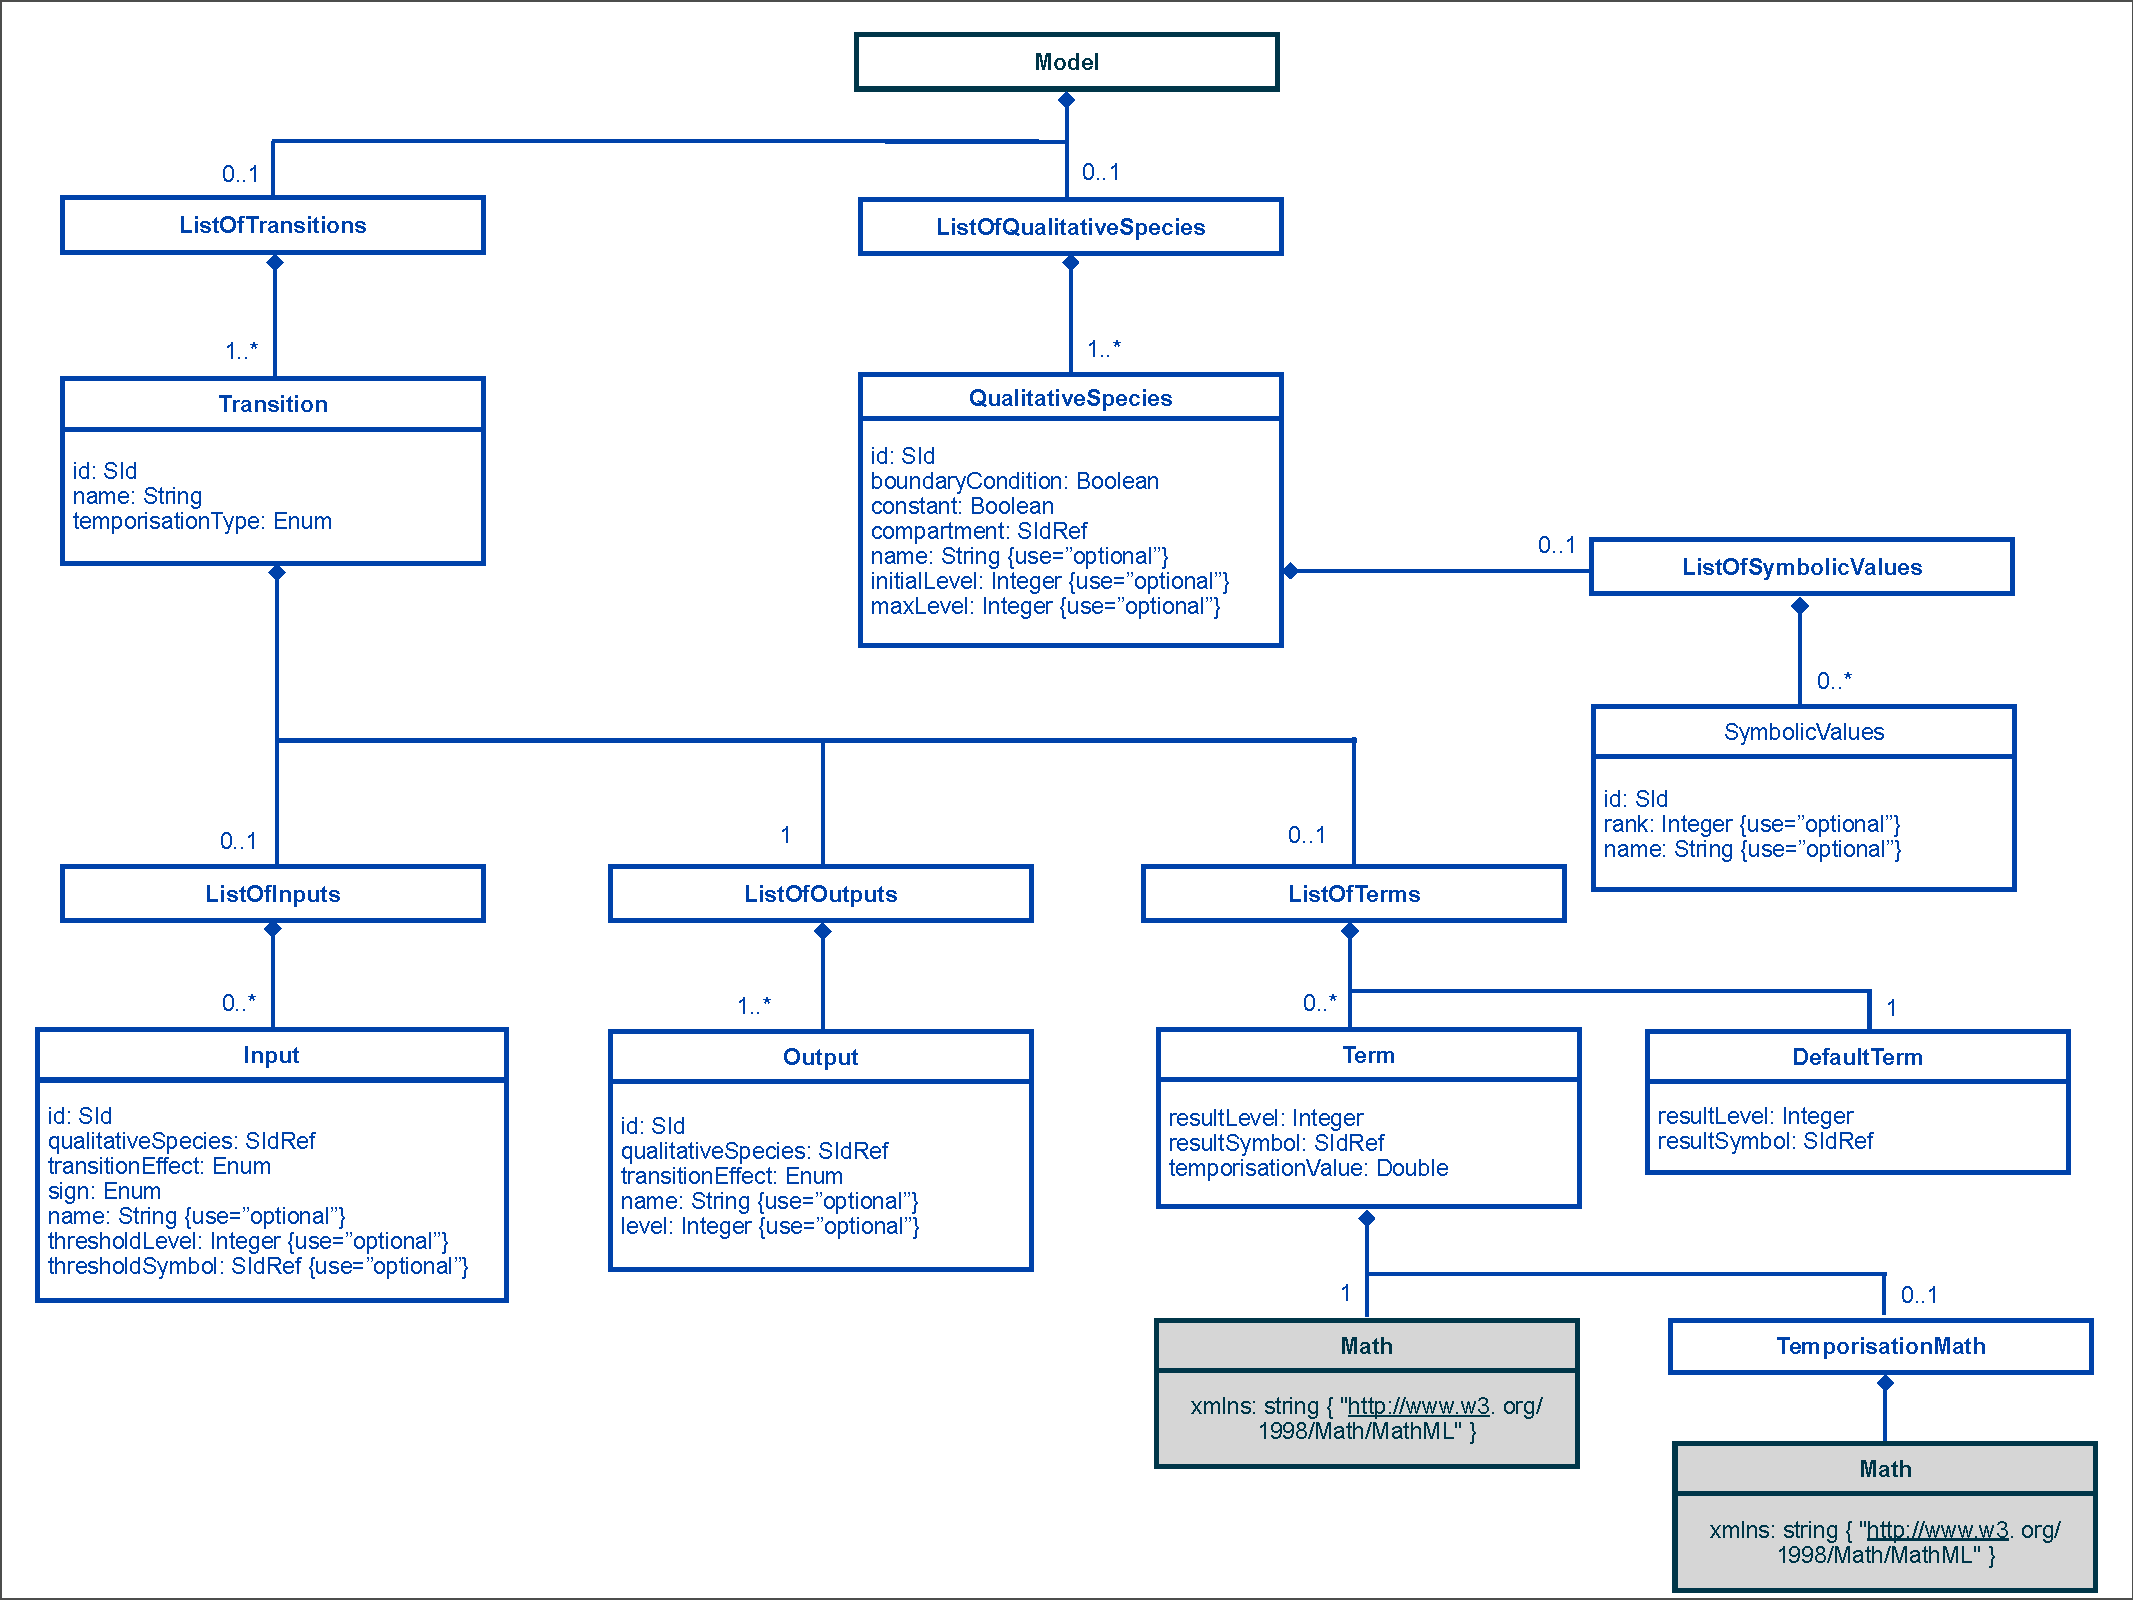
\includegraphics[width=\textwidth]{sbml-proposal-l3f-uml.pdf}
	\end{center}
	\caption{UML diagram of the proposal of Qualitative Models package for SBML Level 3}
	\label{fig:UML}
\end{figure}

% proposed syntax (end)
\bigskip
\subsection*{Extension of the \sbml{Model} element} % (fold)
\label{sub:model}
The SBML element \sbml{Model} is extended to contain at most one \listOf{QualitativeSpecies} and at most one \listOf{Transitions}.
% subsection model (end)
\bigskip
\subsection*{Extension of the \sbml{AssignmentRule} element} % (fold)
\label{sub:AssignmentRule}
The definition of the attribute \attr{variable} of the SBML element \sbml{AssignmentRule} is extended to possibly refer to a \qual{QualitativeSpecies} (in addition to \sbml{Species}, \sbml{SpeciesReference},\sbml{Compartment}, or \sbml{Parameter}). 

% subsection AssignmentRule (end)
\bigskip
\subsection*{Extension of the \sbml{EventAssignment} element} % (fold)
\label{sub:event}
The definition of the attribute \attr{variable} of the SBML element \sbml{EventAssignment} is extended to possibly refer to a \qual{QualitativeSpecies} (in addition to \sbml{Species}, \sbml{SpeciesReference},	\sbml{Compartment}, or \sbml{Parameter}). 

% subsection event (end)
\bigskip
\subsection*{Definition of \textsf{\textbf{\hypertarget{QualitativeSpecies}{QualitativeSpecies}}}} % (fold)

The \sbml{Model} element may contain (at most) one \listOf{QualitativeSpecies} that contains at least one \qual{QualitativeSpecies}.

A \qual{QualitativeSpecies} describes a pool of indistinguishable entities in a \sbml{Compartment}. It is associated with either a \emph{level} or a \emph{symbol} from its \listOf{SymbolicValues}.

\paragraph{The \attr{id} and \attr{name} attributes:}
These attributes are used according to the SBML L3v1 Section 3.3. The attribute \attr{id} is mandatory and \attr{name} is optional. 

\paragraph{The \attr{compartment}, \attr{constant} and \attr{boundaryCondition} attributes:}
These attributes are treated as in \sbml{Species} elements.

\paragraph{The \attr{initialLevel}  attribute:}
The \attr{initialLevel} is an \type{integer} that defines the initial level of the \qual{QualitativeSpecies} in its \sbml{Compartment}. This attribute is optional.

\paragraph{The \attr{maxLevel} attribute:}
The \attr{maxLevel} is an \const{integer} that sets the maximal level of the \qual{QualitativeSpecies}. This attribute is optional.

% subsection qualitativespecies (end)
\bigskip
\subsection*{Definition of \qualt{SymbolicValue}} % (fold)
The \qual{QualitativeSpecies} element may contain at most one \listOf{SymbolicValues} that contains zero or more \qual{SymbolicValue}s. An empty list is allowed, and useful for e.g. adding annotations.
The \qual{SymbolicValue} element defines a non instantiated parameter. Such symbols may represent the different solutions of piecewise linear differential equations, along with different thresholds.

\paragraph{The \attr{id} and \attr{name} attributes}
These attributes are used according to the SBML L3.1 Section 3.3. The attribute \attr{id} is mandatory and \attr{name} is optional. 

\paragraph{The \attr{rank} attribute}
The \attr{rank} is an \type{integer} that defines the position of the symbol in the \listOf{SymbolicValues}. This attribute is optional.

% subsection SymbolicValues (end)
\bigskip
\subsection*{Definition of \qualt{Transition} } % (fold)
The \sbml{Model} element may contain at most one \listOf{Transitions} that contains at least one \qual{Transition}.
A \qual{Transition} element contains at most one \listOf{Inputs}, exactly one \listOf{Outputs} and one \listOf{FunctionTerms}.

\paragraph{The \attr{id} and \attr{name} attributes:}
These attributes are used according to the SBML L3.1 Section 3.3. They are both optional. 

\paragraph{The \attr{temporisationType} attribute:}
The \attr{temporisationType} is an \type{enumeration} the "temporisation" of the \qual{Transition}, that is the updating policy associated with the \qual{Transition}. It can be set to \const{timer}, \const{priority}, \const{sustain}, \const{proportion} or \const{rate}.
This attribute is optional. 
% subsection Transitions (end)

\bigskip
\subsection*{Definition of \qualt{Input}} % (fold)
The \listOf{Inputs} contains zero or more \qual{Input}s. A transition with zero inputs can be useful to define an initial assignment, where the state of an output depends on a function but not on any input values. An empty list is allowed, and useful for e.g. adding annotations.
Each \qual{Input} refers to a \qual{QualitativeSpecies} that participates to the corresponding \qual{Transition}.

\paragraph{The \attr{id} and \attr{name} attributes:}
 These attributes are used according to the SBML L3.1 Section 3.3. They are both optional.

\paragraph{The \attr{qualitativeSpecies} attribute:}
The \attr{qualitativeSpecies} is a \type{SIdRef} referring to a \qual{QualitativeSpecies}. This attribute is mandatory.

\paragraph{The \attr{thresholdLevel} and \attr{thresholdSymbol} attributes:}
The \attr{thresholdLevel} is an \type{integer} and \attr{thresholdSymbol} is a \type{SIdRef}. They are optional and exclusive.

\paragraph{The \attr{transitionEffect} attribute:}
The \attr{transitionEffect} is an \type{enumeration} describing how the \attr{qualitativeSpecies} is affected by the \qual{Transition}. On inputs, the value of \attr{transitionEffect} can be either \const{none} or \const{consumption}. (See section \hyperlink{inter_trans}{Interpreting transitions}). This attribute is mandatory.

\paragraph{The \attr{sign} attribute}
The \attr{sign} is an \type{enumeration} that can be used as an indication on whether the contribution of this input is positive, negative, or both. Thus, possible values can be either \const{positive}, \const{negative} or \const{dual}. The sign is usually used for visualization purposes only. This attribute is optional.

% subsection inputs (end)
\bigskip
\subsection*{Definition of \qualt{Output}} % (fold)
The \listOf{Outputs} contains at least one \qual{Output}.
Each \qual{Output} refers to a \qual{QualitativeSpecies} that participates to the corresponding \qual{Transition}.

\paragraph{The \attr{id} and \attr{name} attributes:}
These attributes are used according to the SBML L3.1 Section 3.3. They are both optional. 

\paragraph{The \attr{qualitativeSpecies} attribute:}
The \attr{qualitativeSpecies} is a \type{SIdRef} referring to a \qual{QualitativeSpecies}. This attribute is mandatory.

\paragraph{The \attr{level} attribute:}
The \attr{level} is an \type{integer} used along with the \attr{transitionEffect} set to \const{production} to specify the effect of the \qual{Transition} on the corresponding \qual{QualitativeSpecies}. This attribute is optional.

\paragraph{The \attr{transitionEffect} attribute:}
The \attr{transitionEffect} is an \type{enumeration} describing how the \attr{qualitativeSpecies} is affected by the \qual{Transition}. On outputs, the value of \attr{transitionEffect} can be \const{production}, \const{assignmentLevel} or \const{assignmentSymbol}. (See section \hyperlink{inter_trans}{Interpreting transitions}). This attribute is mandatory.

% subsection outputs (end)
\bigskip
\subsection*{Definitions of \qualt{FunctionTerm} and \qualt{DefaultTerm}} % (fold)
The \listOf{FunctionTerms} may contain any number of \qual{FunctionTerm} elements, and exactly one \qual{DefaultTerm}. Each term is associated with a result (symbolic or level) and a \qual{FunctionTerm} is associated with a Boolean function inside a \sbml{Math} element. The disjunction of the terms defines the \emph{qualitative function} associated with a \qual{Transition}.

\paragraph{The \attr{resultLevel} and \attr{resultSymbol} attributes:}
The result of the term is described by a \attr{resultLevel} or a \attr{resultSymbol}. Both are optional, but one of them must be defined.

The \attr{resultLevel} is an \type{integer} describing a level. The \attr{resultSymbol} is a \type{SIdRef} referring to a \qual{SymbolicValue}.

\paragraph{The \attr{temporisationValue} attribute and the \sbml{TemporisationMath} element:}
The attribute \attr{temporisationValue} and the element \sbml{TemporisationMath} allow the specification of the "temporisation" of the \qual{Transition} under the corresponding \qual{FunctionTerm}. Both are optional. Depending on the value of the \attr{temporisationType}, either one or both could be used.

The \attr{temporisationValue} is a \type{double}. The element \sbml{TemporisationMath} holds a MathML function returning a \type{double}. 

\paragraph{The \sbml{Math} element:}
Each \qual{FunctionTerm} holds a Boolean function encoded in a \sbml{Math} element, using the subset of MathML 2.0 as defined in SBML L3v1 Section 3.4.6.
This element encodes the conditions under which the \qual{FunctionTerm} is selected.


% subsection Terms (end)
\bigskip
\subsection*{\hypertarget{inter_trans}{Interpreting transitions}} % (fold)

\paragraph{Determining the result of a qualitative function:}
The qualitative function associated with a \qual{Transition} is encoded by a \listOf{FunctionTerms}. The \qual{Transition} contains exactly one \qual{DefaultTerm} describing the result of the function by default. A \qual{FunctionTerm} in a \qual{Transition} defines a result (\attr{resultLevel} or \attr{resultSymbol}) as well as the conditions (\sbml{Math} element) under which this \qual{FunctionTerm} is selected.
The conditions are encoded in MathML as a Boolean function that returns \const{true} if the conditions are fulfilled.
Several \qual{FunctionTerm} elements can have the same result; the qualitative function is then defined as the disjunction of their conditions. 

\paragraph{Encoding the conditions:}
To encode the conditions of the qualitative function, one can use \mathml{ci} elements of MathML to refer to SBML elements. A \mathml{ci} referring to the \attr{id} of a \qual{QualitativeSpecies} then refers to the level or the symbol of this \qual{QualitativeSpecies}, while a \mathml{ci} referring to the \attr{id} of an \qual{Input} then refers to the \attr{thresholdLevel} or the \attr{thresholdSymbol} of this \qual{Input}.


\paragraph{The transitionEffect:}
The \qual{Input} and \qual{Output} elements refer to a \qual{QualitativeSpecies} using the attribute \attr{qualitativeSpecies}. They are defined with a \attr{transitionEffect} attribute that takes one of the following values :
\begin{itemize}
	\item \const{none}: Neither the level nor the symbol associated to the \attr{qualitativeSpecies} is modified.
	\item \const{consumption}: The level of the \attr{qualitativeSpecies} is decreased by the \attr{resultLevel} of the selected term possibly modified by the \attr{thresholdLevel} of the \qual{Input}.
	\item \const{production}: The level of the \attr{qualitativeSpecies} is increased by the \attr{resultLevel} of the selected term possibly modified by the \attr{level} of the \qual{Output}.
	\item \const{assignmentLevel}: The level of the \attr{qualitativeSpecies} is set to the \attr{resultLevel} of the selected term.
	\item \const{assignmentSymbol}: The symbol associated to the \attr{qualitativeSpecies} is set to the \attr{resultSymbol} of the selected term.
\end{itemize}

% subsection interpreting (end)

\section{Use-cases and examples} % (fold)
\bigskip
\subsection*{Simple Logical Regulatory Graph} % (fold)
\label{sub:lrg}
\LRG The following example shows a simple LRG with 3 regulators A, B and C, where A can take three values ($A=\{0,1,2\}$), and B,C are Boolean. The logical functions are the following : $B := 1\ if\ A \ge 1$, $C := 1\ if\ B \ge 1$, $A := 2\ if\ (A \ge 1\ and\ A < 2)\ or\ C \ge 1 ; A := 1\ if\ A < 1\ and\ C \ge 1 ; A := 0\  otherwise$.

\lstinputlisting[caption=Logical Regulatory Graph example,label=ex_LRG]{Examples/example.sbml}

% subsection lrg (end)
\bigskip
\subsection*{Simple Petri net} % (fold)
\label{sub:ex_pn}
\PN The following example shows a simple Petri net, containing 4 places A, B, C and D with one transition $t1$.

\lstinputlisting[caption=Petri net example,label=ex_pn_listing]{Examples/examplePetri.sbml}

% subsection ex_pn (end)

% section use-cases and examples (end)
\section{Package dependencies} % (fold)
This package does not depend on any other SBML Level 3 package.
% section package dependencies (end)
\section{Prototype implementations} % (fold)
Prototype for GINsim.
% section prototype implementations (end)
\section{Unresolved issues} % (fold)
% section unresolved issues (end)
\section{Recommended Practices} % (fold)
\ALL To be valid, the SBML root element must express the requirement of this package: \texttt{<sbml $\dots$ qual:required="true" $\dots$ >}.

\medskip
\PN In Petri nets the initial conditions are part of the model, the \attr{initialLevel} must be defined.
To represent unbounded places, the \attr{maxLevel} should be not specified.

\medskip
\LRG Discussions are still ongoing about the possible (but some times convenient to avoid cumbersome descriptions) incoherency of the \qual{FunctionTerm} elements. For the moment, here are the guidelines to ensure coherent definitions:
\begin{itemize}
\item The \qual{FunctionTerm} elements of all the transitions targeting the same output should be "coherent": the conditions of two \qual{FunctionTerm} elements, leading to different effects on the level/symbol of the output, should not be fulfilled at the same time( i.e. they should be exclusive).
\item If several \qual{FunctionTerm} elements lead to the same effect on the level/symbol of the same output, then the importing tool should consider the disjunction (OR) on the conditions of the terms. 
\end{itemize}

\medskip
\LRG To declare external nodes (ones that have no Boolean expression/truth table associated with them), one should set the attribute \attr{boundaryCondition} of the  \qual{QualitativeSpecies} to TRUE: 
\begin{verbatim}
<qualitativeSpecies id="EGF" maxLevel="1" boundaryCoundition="true" 
                                                  compartment="extracellular"/> 
\end{verbatim}

%Thus, the  \qual{QualitativeSpecies} is defined as being in the boundary on the  system, and cannot be used as an output in any transition."
\medskip
\LRG To declare a "delay" node, which is specified to delay its state update for $k$ iterations, one should set, for all the \qual{Transition} elements having this node as their (unique) output, the attribute \attr{temporisationType} to the value \const{timer} and the \attr{temporisationValue} to $k$. 

\medskip
\LRG To declare a "sustain" node, which is specified to sustain (i.e., to remain in) its latest state for the next $k$ iterations, one should set, for all the \qual{Transition} elements having this node as their (unique) output, the attribute \attr{temporisationType} to the value \const{sustain} and the \attr{temporisationValue} to $k$. 


% section recommended Practices (end)
\section*{References} % (fold)
% section references (end)
\section*{Appendix} % (fold)
% section appendix (end)

\end{document}